\section{Auswertung}
\subsection{Entladungsstrom}\label{sec:Entladungsstrom}
In diesem Versuchsteil soll die Abhängigkeit des Entladungsstroms  $I_{\mathrm{D}}$ von der Entladungsspannung $U_{\mathrm{D}}$, Heizstrom $I_{\mathrm{H}}$ und dem Druck $p$ untersucht werden. Dazu wird jeweils einer der Paramter variiert und die Werte der beiden anderen Paramter werden nicht verändert. Die Messung wird durch geführt mit eingeschaltetem bzw. ausgeschaltetem  zweitem Filament in der target Kammer. Die Ergebnisse sind in den Abbildungen \ref{fig:3_1_Spannung}, \ref{fig:3_1_Strom} und \ref{fig:3_1_Druck} dargestellt. Für die Fehlerbalken sind die folgenden Fehler angenommen: $\Delta U_{\mathrm{D}} = 0.2 $ V, $\Delta I_{\mathrm{H}} = 0.02$ A, $\Delta I_{\mathrm{D}} = 0.02$ A und  $\Delta p = 0.2 $ mm. Da das Druckmessgerät kaputt war, konnte der Druck nicht gemessen werden. Der Druck ist deshalb angegeben in der Skala des Ventils, das den Gaszufluss in den Doppel Plasma Apparat regelt. Der Zusammenhang zwischen dieser Skala (in mm) und dem tatsächlichen Druck ist nicht bekannt, deshalb kann daraus der tatsächliche Druck nicht berechnet werden. Die Abhängigkeit des Entladungsstroms von der Entladungsspannung mit eingeschaltetem und ausgeschaltetem 2. Filament ist in der Abbildung \ref{fig:3_1_Spannung} dargestellt. Der konstant gehaltenne Heizstrom beträgt $ I_{\mathrm{H}} =6.00$ A für beide Sonden, für den Fall das sie eingeschaltet sind. Die Messwerte beider Messungen ähneln sich. Bei kleineren Spannungen als ca \SI{20}{V} ist der Entladungsstrom im Rahmen der Messgenauigkeit null. Bei größeren Werten kommt es erst zu einem sehr starkem Anstieg und danach ändert sich der Entladungsstrom fast nicht mehr. Der Unterscheid hervorgerufen durch das 2. Filament ist, dass mit eingeschaltetem zweitem Filament der Entladungstrom größere Werte annimmmt, bei gleicher Entladunsgspannung.  
\begin{figure}[H]
\centering
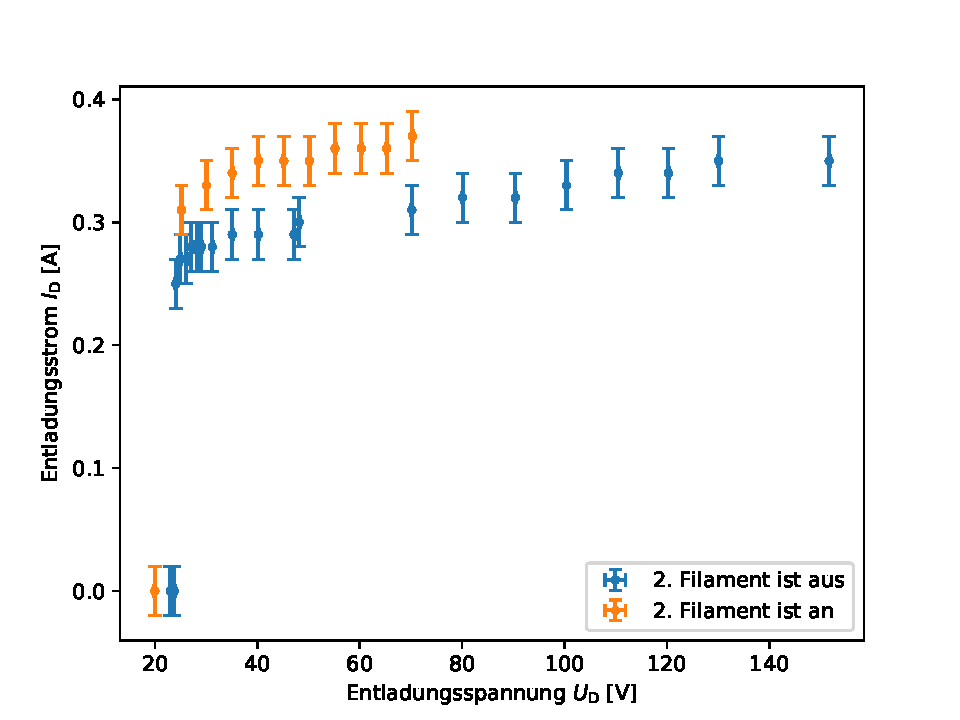
\includegraphics[scale=0.6]{3_1_Spannung.pdf}
\caption{Der Entladungstrom $I_{\mathrm{D}}$ als Funktion der Entladungsspannung $U_{\mathrm{D}}$   mit eingeschaltetem und ausgeschaltetem zweitem Filament in der target Kammer.}
\label{fig:3_1_Spannung}
\end{figure}
In der Abbildung \ref{fig:3_1_Strom} ist die Abhängigkeit des Entladungsstroms von dem Heizstrom mit eingeschaltetem und ausgeschaltete zweitem Filament dargestellt. Die konstant gehaltene Entladungsspannung beträgt $U_{\mathrm{D}}=80.3$ V in dem Fall des ausgeschaltetem zweitem Filament und  ist und $U_{\mathrm{D}}=50.3$ V für den Fall des eingeschaltetem zweitem Filament.   Die Messwerte mit eingeschaltetem und ausgeschaltetem zweitem Filament unterscheiden sich im Rahmen der Messgenauigkeit nicht voneinander. Mit steigendem Heisstrom steigt auch de Entladungsstrom an. Die ursache dafür ist, dass aufgrund des höheren Heizstroms die Temperatur des Filaments ansteigt und somit mehr Elektronen emmitiert werden. 
\begin{figure}[H]
\centering
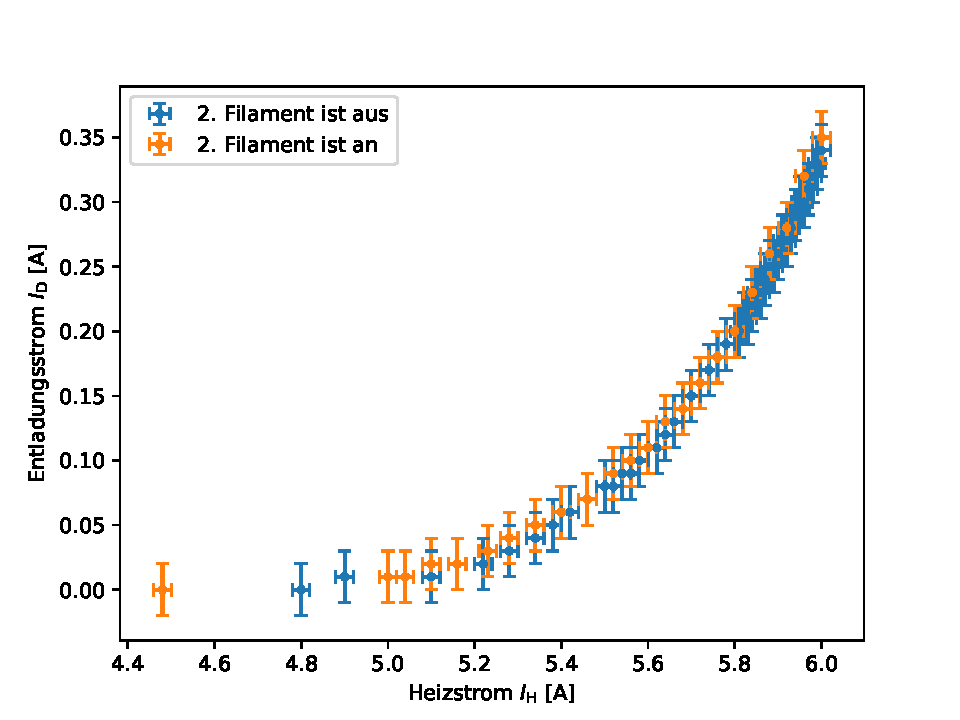
\includegraphics[scale=0.6]{3_1_Strom.pdf}
\caption{Der Entladungstrom $I_{\mathrm{D}}$ als Funktion des Heizstrom $I_{\mathrm{H}}$  mit eingeschaltetem und ausgeschaltetem zweitem Filament in der target Kammer.}
\label{fig:3_1_Strom}
\end{figure}
Der Entladungsstrom als Funktion des Druckes mit eingeschaltetem und ausgeschaltetem zweitem Filament ist in der Abbildung \ref{fig:3_1_Druck} dargestellt. Der konstant gehalteten Heizstrom beträgt $ I_{\mathrm{H}} =6.00$ A und die Entladungsspannung beträgt $U_{\mathrm{D}}=50.2$ V. In dem Bereich \SI{5}{mm} bis ca. \SI{8}{mm} gibt es nur kleine Unterschiede, zwischen eingeschaltetem und ausgeschaltetem zweitem Filament. Der Entladungsstrom steigt zunächst mit steigendem Druck an, bie bei ca \SI{6}{mm} ein Maximum erreicht wird und sinkt danach wieder ab. Mit eingeschaltetem zweitem Filament sinkt der Entladungsstrom auch für größere Werte als \SI{8}{mm} weiter. Mit ausgeschaltetem zweitem Filament dagegen steigt der Entladungsstrom wieder an. Bei ca. \SI{9}{mm} gibt es ein Minimum im Entladungsstrom. 
\begin{figure}[H]
\centering
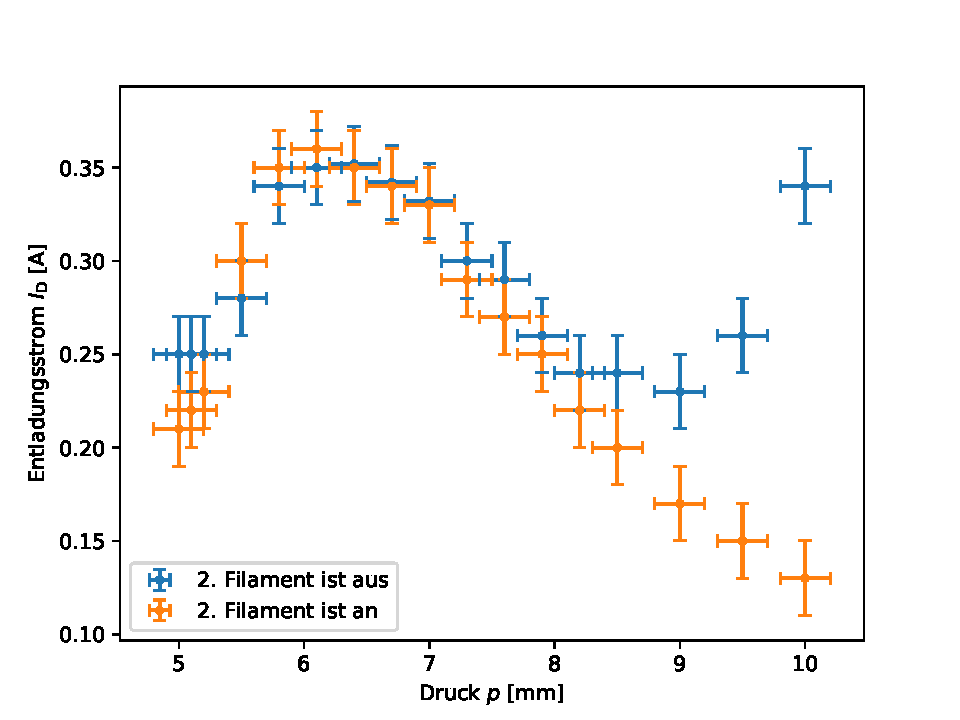
\includegraphics[scale=0.6]{3_1_Druck.pdf}
\caption{Der Entladungstrom $I_{\mathrm{D}}$ als Funktion des Druckes $p$ mit eingeschaltetem und ausgeschaltetem zweitem Filament in der target Kammer.}
\label{fig:3_1_Druck}
\end{figure}
\subsection{Plasma Oszillations Methode}
Mithilfe der Plasma  Oszillations Methode kann die Plasmadichte bestimmt werden. Die Oszillationen werden mit der Langmuir-Sonde gemessen und mit einem Spektrumanalysator dargestellt. Als erstes muss das richtige Maximum gefunden werden. Dazu müssen die Parameter variiert werden. Das Maxima das sich als einziges verändern lässt, ist das gesuchte Maximum. Die Plasmafrequenz kann dann mit dem Spektrumanalysator ermittelt werden. Zu beachten ist, das die Frequnz $f_{\mathrm{p}}$ gemessen wird, die Plasmafrequnz aber normalerweise als Kreisfrequenz angegeben wird: $\omega_{\mathrm{p}}= 2 \pi f_{\mathrm{p}}$.  Aus der Plasmafrequenz  kann dann die Plasmadichte berechnet werden:
\begin{align}
  \omega_{\mathrm{p}}=\sqrt{\frac{e^2 n}{\epsilon_0 m_{\mathrm{e}}}} = 56.5 \sqrt{n}
\end{align}
Durch Umstellen der Gleichung erhält man
\begin{align}
  n=\left( \frac{\omega_{\mathrm{p}}}{56.5} \right)^2=\left( \frac{2 \pi f_{\mathrm{p}}}{56.5} \right)^2.
 \end{align}
Der Fehler kann durch Fehlerfortpfalnzung berechnet werden, wobei als Fehler der gemessenen Frequenz  $\Delta f= 5$ MHz angenommen wird.  
\begin{align}
  \Delta n &= \frac{\mathrm{d} n}{\mathrm{d} f} \Delta f \\
  &=\left( \frac{2 \pi}{56.5} \right)^2 2 f_{\mathrm{p}} \Delta f
\end{align}
Analog zum Kapitel \ref{sec:Entladungsstrom} wird die Abhängigkeit der Plasmadichte von den Parametern Entladungsspannung, Heizstrom und Druck bestimmt. Die Plasmadichte als Funktion der Entladungsspannung ist in der Abbildung \ref{fig:3_2_Spannung dargestellt}. Die Plasmadichte steigt mit steigender Entladungsspannung an. Bei ca. \SI{80}{A} Entladungsspannung kommt es zu eienm Sattelpunkt. Danach steigt die Plasmadichte wieder an. 
\begin{figure}[H]
\centering
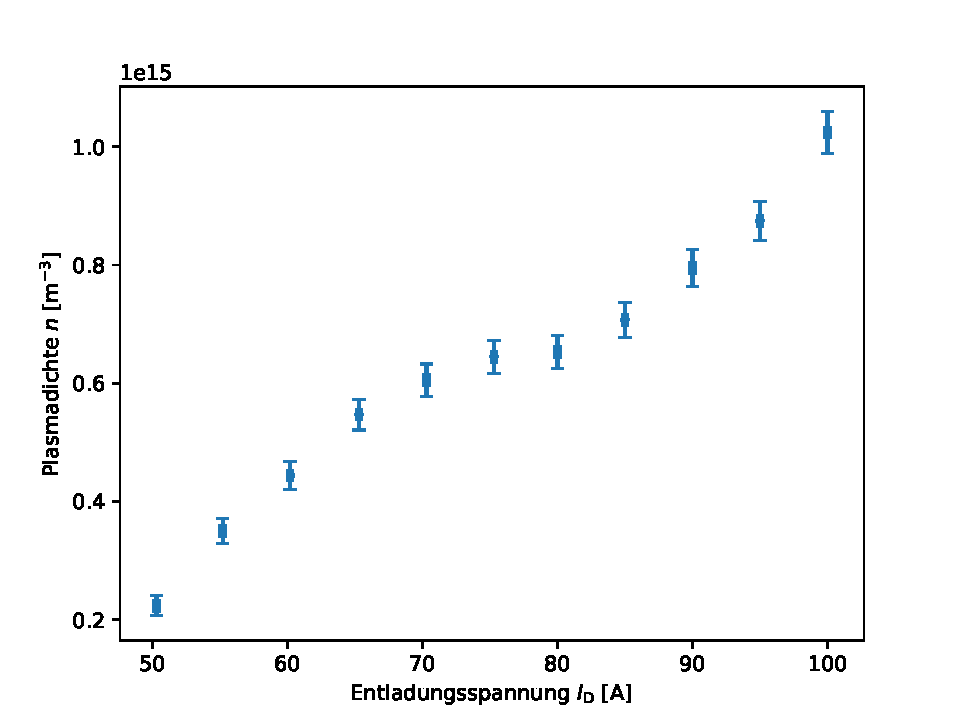
\includegraphics[scale=0.6]{3_2_Spannung.pdf}
\caption{Die Plasmadichte  als Funktion der Entladungsspannung.}
\label{fig:3_2_Spannung}
\end{figure}
Die Plasmadichte als Funktion des Heizstroms ist in der Abbildung \ref{fig:3_2_Strom} dargestellt. Zu erkenne ist  näherungsweisev ein linearer Zusammenhang zwischen dem Heizstrom und der Plesmadichte.  
\begin{figure}[H]
\centering
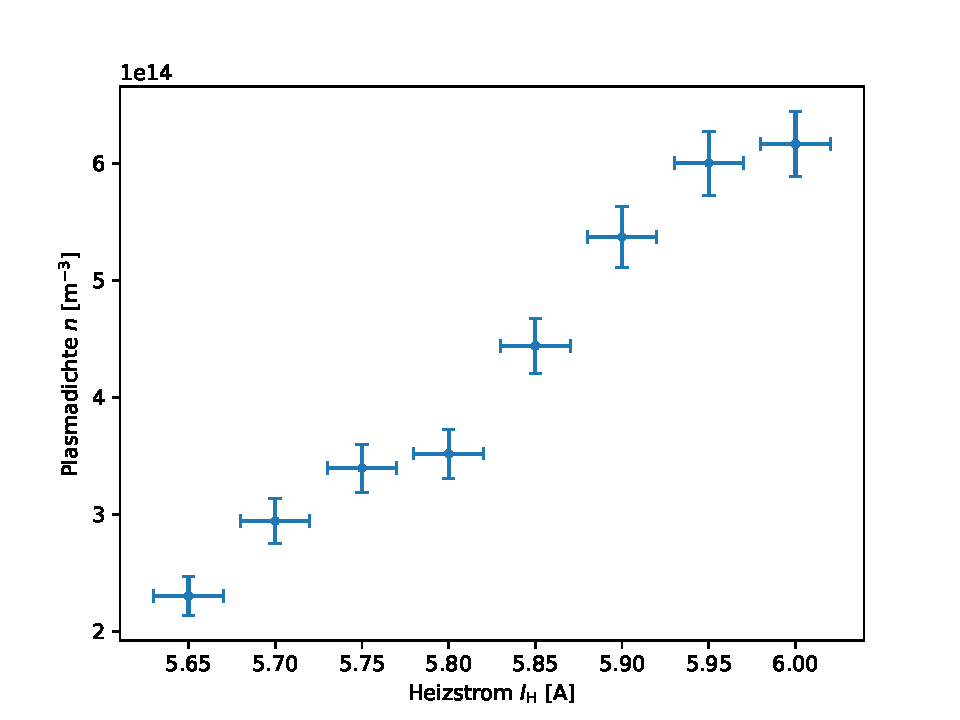
\includegraphics[scale=0.6]{3_2_Strom.pdf}
\caption{Die Plasmadichte als Funktion des Heizstroms.}
\label{fig:3_2_Strom}
\end{figure}
Die Plasmadichte in Abhängigkeit des Druckesist in de Abbildung \ref{fig:3_2_Druck} dargestellt. Die Plasmadichte ist bis ca. \SI{5}{mm} fast konstant. Danach gibt es einen sehr starken Anstieg. Ob dieser Verlauf den Zusammenhang zwischen Druck und Plasmadichte korrekt beschreibt kann nicht untersucht werden, da wie bereits erwähnt das Druckmessgerät kaputt ist. 
\begin{figure}[H]
\centering
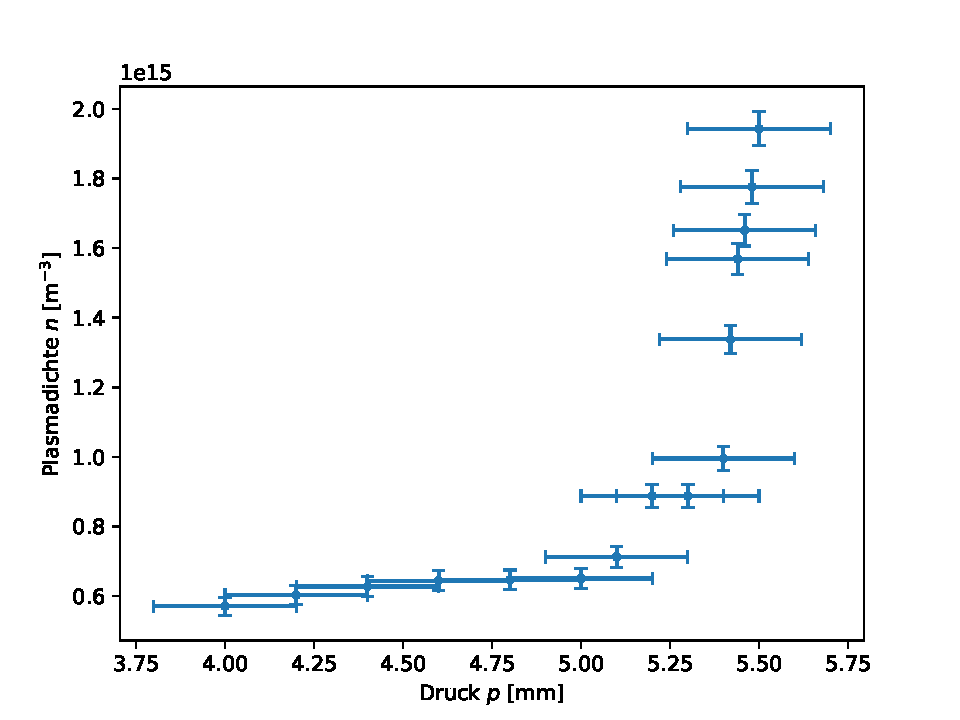
\includegraphics[scale=0.6]{3_2_Druck.pdf}
\caption{Die Plasmadichte als Funktion des Drucks.}
\label{fig:3_2_Druck}
\end{figure}
In allen drei Diagrammen für die Plasmadichte  \ref{fig:3_2_Spannung}, \ref{fig:3_2_Strom} und  \ref{fig:3_2_Druck} liegt die Plasmadicht immer im Bereich von $n=10^{14}\ \frac{1}{\mathrm{m}^3}$ bis  $n=10^{15}\ \frac{1}{\mathrm{m}^3}$.
